\documentclass{article}
\newcommand{\ImageWidth}{11cm}
\newcommand{\blindfootnote}[1]{{\renewcommand\thefootnote{}\footnotetext{#1}}}
\usepackage{tikz}
\usetikzlibrary{decorations.pathreplacing,positioning, arrows.meta}

\begin{document}    

     
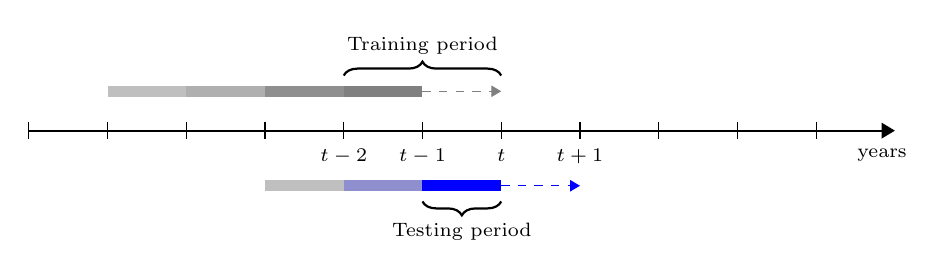
\begin{tikzpicture}
% draw horizontal line   
\draw[thick, -Triangle] (0,0) -- (\ImageWidth,0) node[font=\scriptsize,below left=3pt and -8pt]{years};

% draw vertical lines
\foreach \x in {0,1,...,10}
\draw (\x cm,3pt) -- (\x cm,-3pt);

\foreach \x/\descr in {4/t-2,5/t-1,6/t,7/t+1}
\node[font=\scriptsize, text height=1.75ex,
text depth=.5ex] at (\x,-.3) {$\descr$};

\foreach \x/\perccol in
{1/100,2/75,3/25,4/0}
\draw[lightgray!\perccol!gray, line width=4pt] 
(\x,.5) -- +(1,0);
\draw[-Triangle, dashed, gray] (5,.5) --  +(1,0);

\foreach \x/\perccol in
{3/100,4/75,5/0}
\draw[lightgray!\perccol!blue, line width=4pt] 
(\x,-.7) -- +(1,0);
\draw[-Triangle, dashed, blue] (6,-.7) --  +(1,0);

\draw [thick ,decorate,decoration={brace,amplitude=5pt}] (4,0.7)  -- +(2,0) 
       node [black,midway,above=4pt, font=\scriptsize] {Training period};
\draw [thick,decorate,decoration={brace,amplitude=5pt}] (6,-.9) -- +(-1,0)
       node [black,midway,font=\scriptsize, below=4pt] {Testing period};

\end{tikzpicture}\blindfootnote{Original source here: https://tex.stackexchange.com/questions/436259/timeline-in-latex}

\end{document}